\documentclass[aps,pre,twocolumn,superscriptaddress,floatfix]{revtex4-2}

\usepackage{amsmath,amssymb}
\usepackage{graphicx}
\usepackage{booktabs}
\usepackage{bm}
\usepackage[colorlinks=true,allcolors=blue]{hyperref}

\newcommand{\Ut}{U_{3}}
\newcommand{\Up}{U_{2}}
\newcommand{\eps}{\epsilon}
\newcommand{\TODO}[1]{\textbf{[#1]}}

\begin{document}

\title{Borromean trimers on the Bethe lattice}

\author{Alexei Vazquez}
\email{alexei@nodeslinks.com}
\affiliation{Nodes \& Links Ltd, Salisbury House, Station Road, Cambridge, CB1 2LA, UK}
\date{\today}

\begin{abstract}
Three particles can be bound when no two of them are. On a lattice this
Borromean binding of three distinguishable particles with on-site
attraction $U$ and hopping $t$ is known from Mattis and Rudin; I revisit
it on the Bethe lattice, the infinite tree that random regular graphs
resemble locally, and find that the tree adds one thing a lattice cannot
have. On a non-amenable graph a composite has two binding thresholds,
one for a square-summable state and one for a state whose centre of mass
is the uniform Perron mode, which the spectral gap places below the band;
and quantum statistics selects which one a many-body phase sees, since a
bosonic composite condenses into the Perron mode and binds at the uniform
threshold while a fermionic composite fills a band and binds at the
square-summable one. I compute both thresholds for the pair, in closed
form, and for the trimer, numerically, for branching $K=2$ to $10$. The
trimer binds before the pair in all three comparisons, square-summable
against square-summable, uniform against uniform, and the cross-sector
one that governs the dilute three-flavour gas, a fermionic trimer against
a condensed pair, whose window is $3\%$ of the pair threshold at $K=2$
and $13\%$ at $K=10$. A Fermi liquid of trimers is then the ground state
below a density that vanishes at the trimer threshold. The ordering is
verified on finite random regular graphs; the fermionic no-go of Mattis
follows from an exchange argument that holds on any graph; and a site too
shallow to hold one particle holds three at $0.6$ of the attraction at
which it holds two.
\end{abstract}

\maketitle

\section{Introduction}
Two particles are the unit of the theory of
superconductivity. Three particles are the unit of Efimov physics: with a
resonant two-body interaction, three particles have a tower of bound states
even when no pair is bound~\cite{efimov1970,nielsen2001}, which has been
observed in ultracold caesium~\cite{kraemer2006} and in the helium
trimer~\cite{kunitski2015}. Bound triples without bound pairs, Borromean
states, are also known on lattices, where the band structure replaces the
resonance: on the cubic lattice three distinguishable particles with
on-site attraction bind at an attraction below the pair threshold, while
two identical fermions and a third particle do
not~\cite{mattis1984,mattis1986}. In many-body physics the triple appears
as the trion of three-flavour attractive fermions, the cold-atom analogue
of the baryon, which competes with the colour superfluid of
pairs~\cite{rapp2007,inaba2009,inaba2010} and has a Cooper-problem
analogue, the Cooper triple~\cite{niemann2012,akagami2021,tajima2022}; as
the charge-$6e$ condensate of three bound Cooper pairs~\cite{ge2024}; as
the light clusters of warm nuclear matter, where Pauli blocking
dissolves the deuteron before the triton~\cite{typel2010}; and, as the
ordered-phase cousin of Borromean binding rather than a realisation of
it, as the Borromean super-counterfluid of three-component mixtures, in
which a cubic coupling locks three inter-component phases at once so that
the three-component counterflow is superfluid while no component and no
pair is~\cite{blomquist2021,babaev2024,kuklov2025}.

Random networks are the other place where the pair-versus-triple question
has consequences. A random regular graph is locally a tree, its local
physics in the thermodynamic limit is that of the Bethe lattice of the
same degree, where the cavity method is
exact~\cite{abouchacra1973,vazquez2023pre}, and on that lattice the
attractive Hubbard model has been solved by dynamical mean-field
theory~\cite{keller2001,garg2005,toschi2005}, with
disorder~\cite{ioffe2010,feigelman2010} and with three
flavours~\cite{inaba2009,inaba2010}. Yet the few-body anchor of these
phase diagrams, whether the trion or the pair forms first as the
attraction grows at zero density, is not known on a tree, and a tree
raises a question a lattice does not: its uniform mode is not
square-summable, so a composite has two thresholds, not one.

It helps to say at the outset what in this paper is a new instance of
known physics, what is new as a result of calculation, and what is new
physics. Known, and recovered here on a new graph, are four things: that
a band edge alone produces Borromean binding of three distinguishable
particles, the result of Mattis and Rudin on the cubic
lattice~\cite{mattis1984}; that two identical fermions and a third
particle do not bind, Mattis's no-go~\cite{mattis1986}, which the
exchange argument of Sec.~\ref{sec:fermions} shows to hold on any graph;
that a lattice has no Efimov tower, which was Mattis's point and which
the count of Sec.~\ref{sec:conclusions} confirms; and that the
three-flavour gas has a trionic phase at strong
coupling~\cite{rapp2007,inaba2010}, here extended to zero density with a
point-trimer estimate. New as results of calculation, and useful for the
random-graph and dynamical-mean-field literature, are the closed-form
pair thresholds in both sectors, Eqs.~\eqref{eq:U2}
and~\eqref{eq:U2L2}, their exact large-$K$ limits from the semicircle
density, the monotonic growth of the Borromean window with the degree,
the thresholds at a single deep site and on a disordered tree, and the
direct verification of the ordering on random regular graphs conditioned
on girth. New physics, in the sense of a statement with no lattice
counterpart, is one thing: on a non-amenable graph a composite has two
thresholds, separated by the spectral gap that the Alon--Boppana bound
makes unavoidable~\cite{alon1986,nilli1991}, and quantum statistics
selects which one a many-body phase sees. A bosonic composite condenses
into the Perron mode and binds at the uniform threshold; a fermionic
composite fills a band and binds at the square-summable one.
Section~\ref{sec:density} is the evidence: the chemical potential of the
colour superfluid tends to the uniform-sector pair energy, while the
trimer liquid starts from the square-summable bottom. The window that
governs the dilute phase diagram is therefore the cross-sector one, a
fermionic trimer against a condensed pair, and the ordering holds in all
three comparisons, which is a stronger statement than any one of the
numbers in Table~\ref{tab:thr}.

\section{Model and the two thresholds}
\label{sec:model}
Consider the Bethe lattice of
degree $z=K+1$, the infinite tree in which every vertex has $K+1$
neighbours, with $K$ the branching. Distinguishable particles
$p=1,\dots,m$ hop between neighbouring vertices with amplitude $-t$ and
attract on site,
\begin{equation}
  H=-t\!\sum_{\langle ij\rangle,p}\!
  \left(c^{\dagger}_{ip}c_{jp}+\text{h.c.}\right)
  -U\sum_{i,\,p<q}n_{ip}n_{iq}
  +\sum_{i}\eps_{i}n_{i},
  \label{eq:H}
\end{equation}
where h.c.\ stands for the Hermitian conjugate of the preceding term,
\begin{equation}
  n_{ip}=c^{\dagger}_{ip}c_{ip},\qquad n_{i}=\sum_{p}n_{ip},
  \label{eq:n}
\end{equation}
and $\eps_{i}$ is a site energy, zero except where stated. Figure~\ref{fig:scheme}
shows the setting and the question. For three flavours of
fermions the flavours are the labels $p$ and the statistics plays no role;
I call the three-body bound state a trimer throughout and reserve trion for
the many-body literature. The single-particle spectrum of the tree is the
band $|E|\le2\sqrt{K}\,t$ with the Kesten--McKay density of
states~\cite{kesten1959,mckay1981}, so $m$ free particles have their
continuum edge at $-2m\sqrt{K}\,t$. The constant vector is an eigenvector
of the hopping with energy $-(K+1)t$, below the band, and it is not
square-summable: it is the Perron mode of a finite random regular graph,
where it is a legitimate state. A composite of $m$ particles is bound when
its energy lies below $-2m\sqrt{K}\,t$, and on a tree that can be asked in
two sectors. In the \emph{square-summable} sector the composite is an
ordinary normalisable state, its centre of mass at the band bottom
$-2\sqrt{K}\,t_{\rm eff}$ of its own effective hopping. In the
\emph{uniform} sector the relative motion is normalisable but the centre of
mass is the Perron mode, at $-(K+1)t_{\rm eff}$, lower. The uniform
threshold is therefore the lower of the two. The gap between the Perron
energy $-(K+1)t$ and the band edge $-2\sqrt{K}\,t$ is the spectral gap of
a regular non-amenable graph, which the Alon--Boppana bound makes
unavoidable on any family of $(K+1)$-regular graphs~\cite{alon1986,nilli1991}; on a
lattice the uniform mode is the $P=0$ Bloch state, inside the band, and
the two thresholds coincide. Both are physical, and Sec.~\ref{sec:density}
shows which one a many-body phase sees: a condensate of bosonic
composites occupies the Perron mode and binds at the uniform threshold,
a Fermi liquid of composites fills a band and binds at the
square-summable one. Every number below says which sector it belongs to.
I set $t=1$.


\begin{figure}[t]
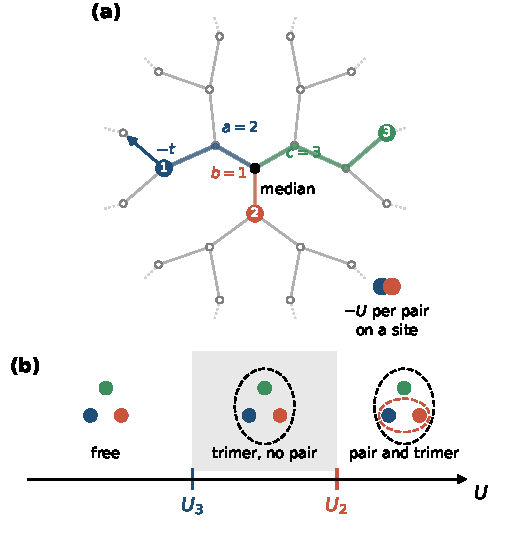
\includegraphics[width=\columnwidth]{fig0.pdf}
\caption{The problem. (a) Three distinguishable particles on the Bethe
lattice of degree $3$ ($K=2$), hopping with amplitude $-t$ and attracting
with $-U$ per pair on a site. The median vertex is the unique vertex on
the three geodesics, and the distances $(a,b,c)$ from it are the
coordinates of the uniform sector, Sec.~\ref{sec:uniform}. (b) The
question is the order of the two thresholds: the attraction $\Ut$ at which
three particles first bind and $\Up$ at which two do. Between them
(shaded) the trimer exists and no pair does, the Borromean window; on a
tree each threshold is asked in two sectors, Sec.~\ref{sec:model}.}
\label{fig:scheme}
\end{figure}

\section{Uniform sector}
\label{sec:uniform}
The tree has a transitive automorphism group,
and the uniform sector is the set of wavefunctions constant on its orbits,
the analogue of zero total momentum. For two particles the orbit is their
distance $d$, with $n_{d}=(K+1)K^{d-1}$ configurations per particle at
$d\ge1$. For three particles the orbit is the triple $(a,b,c)$ of distances
from their median, the unique vertex on all three geodesics, with the
particles at positive distance in distinct branches; the orbit has
$n(a,b,c)=(K+1)^{(k)}K^{a+b+c-k}$ configurations per median, where $k$ is
the number of positive entries and $x^{(k)}$ the falling factorial. The
Hamiltonian acts on orbit functions $f$ through a matrix $M$ of hop
counts, Fig.~\ref{fig:calc}(b), that satisfies detailed balance with
respect to $n$, so $g=\sqrt{n}\,f$
obeys a symmetric problem with kinetic elements $-t\sqrt{M_{ss'}M_{s's}}$.
The two-body sector is a half line in $d$, Fig.~\ref{fig:calc}(a), with
hopping $J=2\sqrt{K}\,t$ for $d\ge1$, hopping $J_{0}=2\sqrt{K+1}\,t$ on the
first link and site energy $-U$ at $d=0$; the cavity element of the half line at the band edge is
$1/J$, and the bound-state condition $-U-E-J_{0}^{2}/J=0$ at $E=-2J$ gives
\begin{equation}
  \Up^{\rm u}=2J-\frac{J_{0}^{2}}{J}=\frac{2(K-1)}{\sqrt{K}}\,t .
  \label{eq:U2}
\end{equation}
\begin{figure}[t]
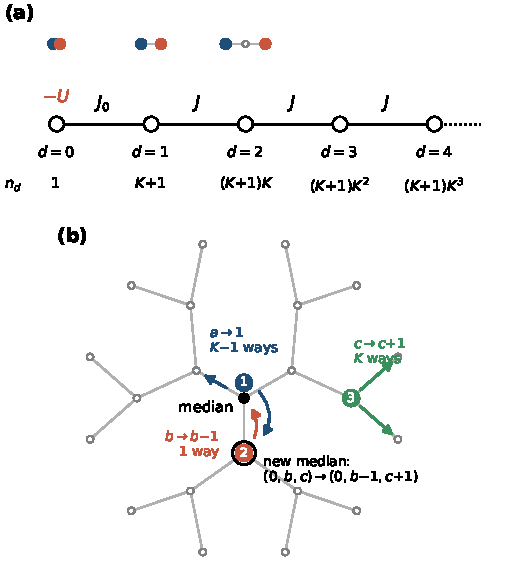
\includegraphics[width=\columnwidth]{fig0b.pdf}
\caption{The uniform-sector calculation. (a) The pair problem reduced to
the half line of the distance $d$: site energy $-U$ at $d=0$, hopping
$J_{0}=2\sqrt{K+1}\,t$ on the first link and $J=2\sqrt{K}\,t$ beyond, with
the orbit sizes $n_{d}$ and, above the first three sites, the
configurations they stand for. (b) The moves in the three-body orbit
$(a,b,c)$, for $K=2$: a particle steps away from the median with $K$
choices or towards it with one; a particle at the median enters a fresh
branch with $K-1$ choices; and a particle at the median stepping towards
another relocates the median (dashed ring), changing two distances at
once. The hop counts $M_{ss'}$ are these multiplicities, and the orbit
sizes $n(a,b,c)$ balance them.}
\label{fig:calc}
\end{figure}

It vanishes on the line, $K=1$, as it must, and at large $U$ the pair
energy is $-U-4(K+1)t^{2}/U$, the on-site shift $-2(K+1)t^{2}/U$ plus the
Perron energy of a pair hopping with amplitude $2t^{2}/U$, which is the
sector speaking. The three-body sector I diagonalise with the orbits
truncated at $a+b+c\le L$. The truncated continuum lies above the true
edge, so the smallest $U$ at which the ground energy drops below
$-6\sqrt{K}\,t$ is an upper bound on $\Ut^{\rm u}$ that decreases with $L$;
it is converged at $L=60$ and unchanged at $120$ and $180$. The reduced
model reproduces exact diagonalisation on a ring at $K=1$ to eight digits,
Eq.~\eqref{eq:U2}, and the large-$U$ expansion
$E_{3}=-3U-3(K+1)t^{2}/(2U)+O(t^{4}/U^{3})$.

\section{Square-summable sector}
\label{sec:l2}
Fix a root vertex and take the
wavefunctions invariant under the automorphisms that fix it, which relabel
the children of every vertex independently. A configuration is reduced to
canonical form by relabelling branches in order of first use along the
particle paths, its orbit measure is a product of falling factorials over
the vertices of the tree spanned by the root and the particles, and the
symmetrisation is as before. Every state in this sector is square-summable
and the sector contains the radial part of every bound state. The
thresholds follow from the Birman--Schwinger principle: with $V$ the
diagonal operator that counts coincident pairs and $H_{0}$ the Hamiltonian
at $U=0$, a bound state below $E$ exists when $U\lambda_{\max}\ge1$, where
$\lambda_{\max}$ is the largest eigenvalue of
$V^{1/2}(H_{0}-E)^{-1}V^{1/2}$, so the threshold is $1/\lambda_{\max}$ at
the edge. For the pair the operator is the propagator between doubly
occupied sites, $b_{d}=\langle ii|(H_{0}+4\sqrt{K}\,t)^{-1}|jj\rangle$ at
distance $d$, a radial kernel and hence a function of the adjacency matrix
of the tree; its norm is its value on the spherical function at the band
edge, and its uniform-sector eigenvalue is its value on the constant
vector,
\begin{equation}
  \frac{1}{\Up}=\sum_{d}b_{d}\,P_{d}(2\sqrt{K}),\qquad
  \frac{1}{\Up^{\rm u}}=\sum_{d}b_{d}\,n_{d},
  \label{eq:U2L2}
\end{equation}
with $P_{d}(2\sqrt{K})=K^{d/2}[(K+1)+d(K-1)]/K$ for $d\ge1$ the distance
polynomial of the tree at the edge. The two thresholds are one kernel read
on two centre-of-mass functions. The $b_{d}$ are a double integral over
the Kesten--McKay density with the spherical functions, the first sum
converges geometrically and gives the pair column of Table~\ref{tab:thr} to
six digits, and the second reproduces Eq.~\eqref{eq:U2}. The trimer has no
such reduction and I compute $\lambda_{\max}$ on the truncated orbit space
at $L=30$ to $60$ and extrapolate with a fitted power of $L$, close to
$2$; the same extrapolation applied to the truncated pair problem
reproduces Eq.~\eqref{eq:U2L2} to $10^{-3}$, and the same routine
reproduces the bisection thresholds of the uniform sector to their grid.

\begin{table}[t]
\caption{Pair and trimer thresholds on the Bethe lattice of branching $K$
(degree $z=K+1$), in units of $t$, in the square-summable sector
($\Up$ from Eq.~\eqref{eq:U2L2}, $\Ut$ extrapolated in $L$,
uncertainty in the last digit) and in the uniform sector ($\Up^{\rm u}$
from Eq.~\eqref{eq:U2}, $\Ut^{\rm u}$ by bisection on a grid of
$2\times10^{-3}$). The last column is the cross-sector ratio of a
square-summable trimer to a uniform pair, the one that governs the
dilute three-flavour gas, Sec.~\ref{sec:density}.}
\label{tab:thr}
\begin{ruledtabular}
\begin{tabular}{rrrrrrrrr}
$K$ & $z$ & $\Up$ & $\Ut$ & $\Ut/\Up$ & $\Up^{\rm u}$ & $\Ut^{\rm u}$ & $\Ut^{\rm u}/\Up^{\rm u}$ & $\Ut/\Up^{\rm u}$ \\
\hline
 2 &  3 & 1.966 & 1.369 & 0.696 & 1.414 & 1.310 & 0.926 & 0.968 \\
 3 &  4 & 3.251 & 2.159 & 0.664 & 2.309 & 2.073 & 0.898 & 0.935 \\
 4 &  5 & 4.269 & 2.741 & 0.642 & 3.000 & 2.637 & 0.879 & 0.914 \\
 5 &  6 & 5.136 & 3.218 & 0.627 & 3.578 & 3.103 & 0.867 & 0.899 \\
 6 &  7 & 5.904 & 3.633 & 0.615 & 4.083 & 3.508 & 0.859 & 0.890 \\
10 & 11 & 8.402 & 4.949 & 0.589 & 5.692 & 4.800 & 0.843 & 0.869 \\
\end{tabular}
\end{ruledtabular}
\end{table}

Table~\ref{tab:thr} and Fig.~\ref{fig:bind} contain the main result. On
every tree with $K\ge2$ the trimer binds before the pair in all three
comparisons: square-summable trimer against square-summable pair, with a
window that widens from $30\%$ of $\Up$ at $K=2$ to $41\%$ at $K=10$;
uniform against uniform, from $7\%$ to $16\%$; and, the comparison that
Sec.~\ref{sec:density} shows to govern the dilute three-flavour gas, a
square-summable trimer against a uniform pair, from $3\%$ to $13\%$. The
first two are the tree's versions of the cubic-lattice result; the third
has no lattice counterpart, and it is the smallest, because the
condensed pair takes the Perron energy while the fermionic trimer does
not. Above $\Up$ the trimer stays below the continuum of a bound pair and
a free particle, $E_{2}(U)-2\sqrt{K}\,t$ in the uniform sector, where the
pair carries the Perron centre of mass and the third particle,
normalisable relative to it, enters at the band edge; so the trimer is
the ground composite for all $U>\Ut$. The large-$K$ limit is the
infinite-coordination limit of dynamical mean-field
theory~\cite{keller2001,garg2005}, with $t^{*}=\sqrt{K}\,t$ fixed and a
semicircular density of states. There the uniform pair threshold is
$\Up^{\rm u}\to2t^{*}$ from Eq.~\eqref{eq:U2}, and the square-summable one
keeps only the $d=0$ term of Eq.~\eqref{eq:U2L2}, since $b_{d}P_{d}$
vanishes as $K^{-d/2}$, so $1/\Up\to b_{0}$ with $b_{0}$ the double
integral of the semicircle at the two-body edge, $\Up\to3.308\,t^{*}$ and
$\Up/\Up^{\rm u}\to1.654$. The trimer ratios of Table~\ref{tab:thr} are
still falling at $K=10$; fits of the form $a+b/\sqrt{K}$ extrapolate them
to about $0.50$ in the square-summable sector, $0.78$ in the uniform one
and $0.79$ across sectors, but the same fit applied to the pair ratio,
whose limit is known, gives $1.54$ for $1.654$, so these are indications
that the infinite-coordination three-flavour gas keeps a finite Borromean
window, not values; the three-body problem on the semicircle is the
calculation that would fix them. On the cubic lattice the same Birman--Schwinger calculation in a
box of relative coordinates gives $\Up=7.914\,t$, the Watson integral, and $\Ut=5.158\,t$
(converged to the last digit at box radius $6$), a window of $35\%$, the
number behind the result of Mattis and Rudin~\cite{mattis1984}. The tree
of degree $6$ has a window of $37\%$ in the square-summable sector, close
to the cubic one, and of $13\%$ in the uniform sector, narrower
because that sector's pair threshold is the lower one.

\begin{figure}[t]
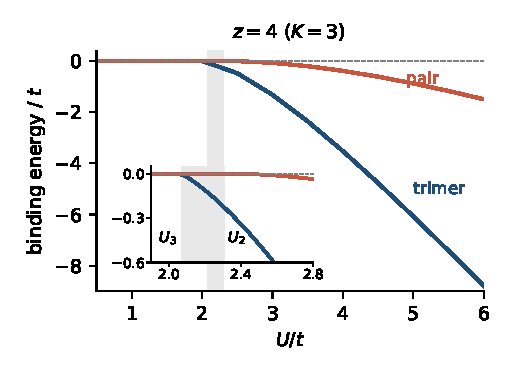
\includegraphics[width=\columnwidth]{fig1.pdf}
\caption{Binding energies in the uniform sector of the Bethe lattice of
degree $z=4$ ($K=3$). Trimer energy measured from the three-particle
continuum edge, $E_{3}+6\sqrt{K}\,t$ (dark line), and pair energy measured
from the two-particle edge, $E_{2}+4\sqrt{K}\,t$ (light line), against the
on-site attraction $U$. The trimer binds at $\Ut^{\rm u}=2.07\,t$, the pair
at $\Up^{\rm u}=2.31\,t$, Eq.~\eqref{eq:U2}. Between the two, shaded, three
particles are bound and no two are.}
\label{fig:bind}
\end{figure}

\section{Finite random regular graphs}
On a finite random regular graph the Perron mode is a normalisable state,
three free particles have their ground state at $-3(K+1)t$, and in the
Borromean window the trimer is not the ground state of three particles but
a state bound relative to the bulk continuum, coupled to the
Perron-containing states with weight $O(1/N)$. To see it I diagonalise
three and two distinguishable particles on random $3$-regular graphs in
the sector orthogonal to the Perron mode on every particle, with a Lanczos
product that applies the projector, and use as diagnostic the probability
that all three particles sit on one site in the three-body ground state
and that both do in the two-body ground state. A bound composite keeps a
finite probability as $N$ grows; an unbound one loses it. Two features of
finite random regular graphs enter. Their lowest bulk states sit on rare
regions, short cycles first, which act as the deep sites of
Sec.~\ref{sec:site} and bind pairs below the clean threshold; I therefore
condition the graphs on girth at least $6$ by rejection sampling. And the
level spacing at the band edge closes only as $N^{-2/3}$, so the approach
to the thermodynamic limit is slow. With that, at $U=1.7\,t$, inside the
square-summable window $1.37<U/t<1.97$, the triple probability is $0.12$,
$0.13$ and $0.14$ at $N=100$, $150$ and $200$, three hundred times its
value at $U=0$, while the pair probability falls from $0.12$ to $0.10$,
$0.08$ and $0.08$ at $N=100$, $200$, $400$ and $800$, six times its
$U=0$ value at $N=100$ and still falling; at $U=2.3\,t$, above $\Up$, the
pair probability is $0.24$ at every $N$, and at $U=1.0\,t$, below both
thresholds, both probabilities fall with $N$. The trimer is bound and the
pair is not, on actual random regular graphs, in the sector the
square-summable thresholds describe.

\section{Finite density}
\label{sec:density}
The two sectors acquire their meaning at finite density, and this section
is the evidence for the claim of the introduction that statistics selects
the sector. A condensate of bosonic composites occupies the Perron mode: the BCS mean field of two
colours with attraction $U$ on the Kesten--McKay density of states, solved
for the gap and the chemical potential $\mu$ at density $n$ per colour, has
$2\mu\to E_{2}^{\rm u}$, the uniform-sector pair energy, as $n\to0$ (to
five digits at $n=10^{-4}$), not the square-summable one. A Fermi liquid
of composites instead fills a band from its square-summable bottom, the
Perron mode being a single state. With three colours the composites are
pairs, which condense, and trimers, which are fermions, so the
zero-density ordering of Table~\ref{tab:thr} asks whether a Fermi liquid
of trimers or a colour superfluid, two colours paired and the third free,
has the lower energy at small $n$, the question that the many-body
literature settles at strong coupling and half
filling~\cite{rapp2007,inaba2010}.

I compare the two at the level of their composites' energies. The trimer is
a point fermion with hopping $t_{3}$ on the tree, defined from the two
sectors' energies at the same $U$ by
$E_{3}-E_{3}^{\rm u}=(K+1-2\sqrt{K})\,t_{3}$, with $E_{3}$ the
square-summable energy extrapolated in $L^{-2}$ from $L=30$ and $45$ and
$E_{3}^{\rm u}$ the uniform one at $L=60$; its band is Kesten--McKay with
bottom $E_{3}$ and its energy per site at density $n$ is that band filled
to $n$. The superfluid is the mean-field energy of the two paired colours
at density $n$ plus a free third colour at $n$. The Hartree energy
$-3Un^{2}$ is common to every uniform phase and is dropped from both. A
mixed phase with a fraction $x$ of the particles in trimers is allowed, and
the ground state is the minimum over $x$. The description holds while the
trimers are dilute on the scale of their size, a few lattice spacings
near threshold, and I use it for $n$ up to $0.1$ per colour.

At zero density the trimer liquid wins for every $U>\Ut$. Between $\Ut$
and $\Up^{\rm u}$ no pair is bound in either sector and the superfluid
reduces to free fermions; above $\Up^{\rm u}$ the trimer lies below a
condensed pair and a free particle, $E_{3}<E_{2}^{\rm u}-2\sqrt{K}\,t$, by
a margin that grows with $U$. The superfluid enters at a density
$n_{1}(U)$ that vanishes at $\Ut$ and rises steeply, Fig.~\ref{fig:phase}:
for $K=2$, $n_{1}=0.003$ at $U=1.38\,t$, $0.015$ at $1.40\,t$, $0.05$
at $1.45\,t$ and $0.09$ at $1.50\,t$, and it crosses $0.1$ at
$U=1.51\,t$; for $K=3$, $n_{1}=0.004$ at $U=2.17\,t$, $0.03$ at $2.20\,t$
and $0.08$ at $2.25\,t$, crossing $0.1$ at $2.26\,t$. The onset is where
the trimer Fermi level reaches the binding energy,
$E_{3}+t_{3}\lambda_{F}(n_{1})=\min(-6\sqrt{K}\,t,\;E_{2}^{\rm u}-2\sqrt{K}\,t)$,
with $\lambda_{F}(n)$ the Fermi level of the Kesten--McKay band at filling
$n$. Above $n_{1}$ the superfluid is a minority component: the trimer band
is narrow, $t_{3}\approx0.17\,t$ at $K=2$ and $0.14\,t$ at $K=3$ near
threshold, so the trimer Fermi level rises slowly and the paired component
takes only the excess, below $3\%$ of the particles at $n=0.1$ and below
$5\%$ at $n=0.3$ for every $U>\Ut$ in the range. The trionic phase of the strong-coupling lattice
gas~\cite{rapp2007,inaba2010} therefore extends to zero density for all
$U>\Ut$, the colour superfluid enters from finite density, and the
zero-density boundary of that phase diagram is the cross-sector
comparison of Table~\ref{tab:thr}: between $\Ut$ and $\Up^{\rm u}$ the
trimer liquid faces no bound pair at all, and above $\Up^{\rm u}$ it
faces a condensed pair whose energy is the uniform-sector one. That is
the window a trion liquid enjoys on a tree, a few per cent at $K=2$ and
$13\%$ at $K=10$, and it is the statement the lattice cannot make. The estimate leaves out the interaction between trimers, the
pairing of the free colour with a trimer's constituents, and the
fluctuations of the mean field; a three-colour cavity calculation at
finite density would fix $n_{1}(U)$ beyond it.

\begin{figure}[t]
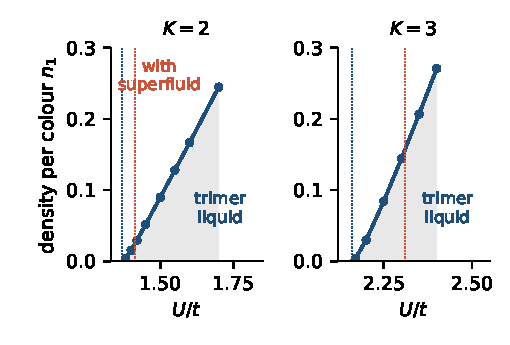
\includegraphics[width=\columnwidth]{fig3.pdf}
\caption{Density $n_{1}$ per colour at which the colour superfluid enters,
against the attraction $U$, for $K=2$ and $3$. Below the line (shaded) a
Fermi liquid of trimers is the ground state; above it the colour
superfluid is a minority component, below $5\%$ of the particles up to
$n=0.3$. The line starts at $\Ut$ and crosses $n=0.1$, the limit of the
composite description, at $U=1.51\,t$ ($K=2$) and $2.26\,t$ ($K=3$).
Dotted lines mark $\Ut$, $\Up^{\rm u}$ and $\Up$ from Table~\ref{tab:thr}.}
\label{fig:phase}
\end{figure}

\section{Two identical fermions}
\label{sec:fermions}
The result depends on the three
particles being distinguishable. In the sector antisymmetric under the
exchange of particles 1 and 2, with attraction only between unlike
particles, the ground energy never drops below the pair-plus-particle
continuum for $U\le14t$ at $K=2$ and $K=3$, and the strong-coupling limit
says why. With the pair on site $i$ and the third fermion on a
neighbour $j$, the hop of the pair's unlike particle to $j$ leaves a pair
at $j$ and a free fermion at $i$, a degenerate configuration, so the
composite moves by exchange at first order in $t$; the fermionic sign
makes the amplitude $+t$, opposite to a hop, and Pauli blocking removes
the site $i$. The relative motion at leading order is the tree with one
vertex removed plus a positive potential $t$ on its neighbours, whose
spectrum lies above $-2\sqrt{K}\,t$, and the pair itself moves only at
order $t^{2}/U$: no bound state. Nothing in this uses the tree. By Cauchy
interlacing the spectrum of any vertex-deleted subgraph lies inside the
band of the graph, and a positive potential raises it, so the argument
recovers Mattis's no-go~\cite{mattis1986} on any graph; the tree adds
nothing to it and the section is a check, not a result. The same exchange with the bosonic sign
$-t$ is what binds trimers in the one-dimensional Bose--Hubbard
model~\cite{valiente2010}, and on the three-dimensional lattice the
equal-mass $2+1$ problem has no discrete spectrum below the continuum at
strong coupling, a trimer requiring a mass ratio above a
threshold~\cite{abdullaev2026}, as in free
space~\cite{kartavtsev2007}. The Borromean trimer of the tree is a
three-flavour object.

\section{One deep site}
\label{sec:site}
Disorder enters at zero density through its
rare sites. Give the root the energy $\eps_{0}<0$: a static impurity is a
fourth particle that does not hop, the root-fixed sector is the natural
one, and its bound states are localised at the impurity. One particle
binds when $|\eps_{0}|>\eps_{c}=(K-1)t/\sqrt{K}$, from
$\eps_{0}-E-(K+1)t^{2}\mathcal{G}(E)=0$ with $\mathcal{G}$ the cavity
resolvent of the clean tree at the band edge, and the reduced model
reproduces this threshold, the impurity energy, and exact diagonalisation
on finite Cayley trees to five digits. For $-\eps_{c}<\eps_{0}<0$ the site
is too shallow to hold one particle, and Fig.~\ref{fig:imp} shows the
attraction it needs to hold two or three. Both thresholds fall from the
square-summable values of Table~\ref{tab:thr} at $\eps_{0}=0$ to zero at
$\eps_{0}=-\eps_{c}$, and the trimer threshold is the lower one at every
depth: $\Ut/\Up$ runs from $0.70$ at $\eps_{0}=0$ through a minimum of
$0.60$ near $0.8\,\eps_{c}$ and back to $0.68$ at $0.99\,\eps_{c}$ for
$K=2$, and from $0.66$ through $0.58$ to $0.65$ for $K=3$.

\begin{figure}[t]
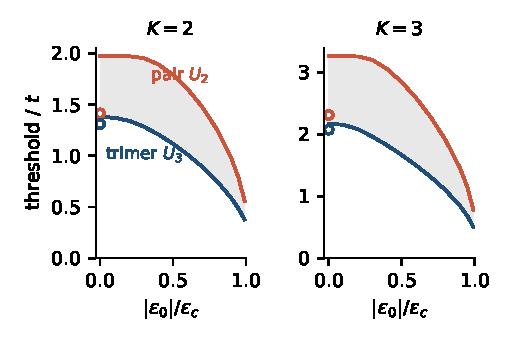
\includegraphics[width=\columnwidth]{fig2.pdf}
\caption{Pair threshold $\Up$ (light line) and trimer threshold $\Ut$
(dark line) at a single site of energy $\eps_{0}$ on the Bethe lattice,
for $K=2$ and $K=3$, against the depth of the site in units of
$\eps_{c}=(K-1)t/\sqrt{K}$, the depth at which one particle binds.
Birman--Schwinger at the continuum edge, orbits truncated at $L=60$ for
the trimer and $120$ for the pair; the change from $L=40$ is below
$0.02\,t$ at $\eps_{0}=0$ and below $0.04\,t$ at $0.99\,\eps_{c}$, where
the states are least localised. Shaded: three particles bound, no two
bound. Open circles at $\eps_{0}=0$: the uniform-sector thresholds of
Table~\ref{tab:thr}.}
\label{fig:imp}
\end{figure}

\section{Disordered tree}
With box disorder $\eps_{i}\in[-W/2,W/2]$ on
every site, the thresholds of Fig.~\ref{fig:imp} classify the sites in
the isolated-site approximation of a Lifshitz tail, each site seen with a
clean environment. For $W=2\eps_{c}$, at $U=0.5\,\Up$ a fraction $0.14$
($K=2$) or $0.17$ ($K=3$) of the sites hold a trimer and no pair, against
$0.05$ or $0.07$ that hold a pair; at $U=0.7\,\Up$ the fractions are
$0.37$ and $0.13$, or $0.35$ and $0.15$; at $W=4\eps_{c}$ a quarter of the
sites hold one particle outright and the Borromean fraction at
$U=0.5\,\Up$ is $0.07$ or $0.09$. The approximation ignores the disorder
around a site, which shifts its thresholds in either direction, and it is
a statement about localised few-body states, not about the many-body
phases; those need the finite-density calculation.

\section{Conclusions}
\label{sec:conclusions}
On the Bethe lattice three distinguishable particles bind before two.
That they do is the band-edge mechanism of Mattis and
Rudin~\cite{mattis1984} on a new graph, and the fermionic no-go and the
absence of an Efimov tower are Mattis's~\cite{mattis1986} as well. What
the tree adds is that a composite on a non-amenable graph has two
thresholds, and that statistics chooses between them: pairs condense
into the Perron mode and bind at the uniform threshold, trimers fill a
band and bind at the square-summable one. The ordering holds in both
sectors and across them, and the cross-sector window, a few per cent at
$K=2$ growing to $13\%$ at $K=10$, is the one a Fermi liquid of trimers
enjoys at low density against a colour superfluid. The exact pair
thresholds, their large-$K$ limits, the growth of the window with the
degree, the deep-site and disorder thresholds and the finite-graph
verification are the calculational content; a shallow site holds three
before it holds two.

The model is realised, with its three flavours, by $^{6}$Li, whose three
lowest hyperfine states have attractions tuned together by a magnetic
field, load into optical lattices, and show their three-body physics in
recombination losses~\cite{ottenstein2008,huckans2009,williams2009}. An
optical lattice is cubic, so what such an experiment tests is the
cubic-lattice window of Mattis and Rudin, $35\%$ by the calculation of
Sec.~\ref{sec:l2}, and not the tree; the tree's specific content, the two
sectors, needs a non-amenable graph. The natural home for that is a
hyperbolic lattice in circuit quantum
electrodynamics~\cite{kollar2019,boettcher2020}, where the separation of
the uniform mode from the bulk band is already the observable and where
the composites, being photonic, are bosonic and see the uniform
thresholds. For electrons the $2+1$ result is a selection rule:
negative-$U$ centres in amorphous
semiconductors~\cite{anderson1975,weaire1971}, which bind spin-paired
electrons, cannot by themselves produce Borromean three-electron centres;
a third flavour, orbital or valley, or a mass imbalance is needed.

For networks the trimer is a dynamically generated higher-order
interaction, a bound triple with no bound pair from a pairwise
Hamiltonian, a hyperedge without its faces~\cite{vazquez2023pre,battiston2020},
of the kind that pairwise inference cannot see.

Last, the Efimov question. The effect is a lattice effect in the sense of
Mattis~\cite{mattis1986}, a consequence of the band edge rather than of a
resonance, and a tower is not expected on a lattice. The count confirms
it: the states below the three-body edge in the uniform sector at
$U=\Up^{\rm u}$, where the pair is at resonance, number one for $K=2$ and
$3$, unchanged from $L=60$ to $180$, with the next state approaching the
edge as $L^{-2}$, a continuum state. The square-summable sector cannot be
used for this count, since the centre-of-mass band of the bound trimer
fills the region below the edge.

\begin{acknowledgments}
All code that produced the numbers in this paper is available at
Ref.~\cite{code}. The calculations were assisted by Claude, an AI
assistant developed by Anthropic. Nodes \& Links Ltd provided support in
the form of salary for Alexei Vazquez but did not have any additional role
in the conceptualization of the study, the analysis, the decision to
publish or the preparation of the manuscript.
\end{acknowledgments}

\bibliographystyle{apsrev4-2}
\bibliography{refs}

\end{document}
